\cleardoublepage


\chapter{Inverse Kinematik}\label{ch:inverse-kinematik}

In der direkte Kinematik wird aus den Gelenkzuständen Position und Rotation des Endeffektors bestimmt.
Der umgekehrte Vorgang, also das Berechnen der Gelenkpositionen bei gegebener Zieltransformation, wird als inverse Kinematik bezeichnet.
Dies ist erforderlich, um Aufgaben in der Umgebung des Roboters zu lösen und die angestrebten Zielpunkte zu erreichen.
Dabei muss beachtet werden, dass oft mehrere gleichwertige Lösungen für eine Zielstellung des Endeffektors vorliegen und die inverse Kinematik offener Ketten oft nicht einfach direkt mithilfe einer mathematischen Formel gelöst werden kann (siehe Abschnitt~\ref{sec:analytische-losung}).
Um die Gelenkwinkel zu erhalten, kann eine Lösung prinzipiell analytisch, numerisch oder geometrisch ermittelt werden.
Die Vor- und Nachteile, sowie die Berechnung dieser Methoden wird in diesem Kapitel näher erläutert.


\section{Analytische Lösung}\label{sec:analytische-losung}

Für eine direkte Lösung muss zunächst die Formel aus Gleichung~\ref{eq:dh5} oder~\ref{eq:alt-tf} herangezogen werden.
Nach Multiplikation der Transformationsmatrizen müsste die entstehende Gleichung~\ref{eq:inv-kin1} nach den freien Variablen $\theta_1$ bis $\theta_n$ bzw. $d_1$ bis $d_n$ aufgelöst werden.
Da aufgrund der rotatorischen Gelenke nichtlineare trigonometrische Funktionen verwendet werden, ist diese Funktion bei Industrierobotern überwiegend nichtlinear und in vielen Fällen auch nicht lösbar.

\begin{equation}
    T_{0,n}(\overrightarrow{q}) = \prod_{i=1}^{n} T_{i-1,i}(q_i)     \label{eq:inv-kin1}
\end{equation}

Im Falle des UR5 ist dieser Ansatz aufgrund der oben genannten Einwände nicht anwendbar und wird an dieser Stelle deshalb nicht detailliert ausgeführt.


\section{Numerische Lösung}

?? Quelle
%?? alt methode file:///home/julin/Downloads/MScThesis\_Marco\_de\_Gier.pdf

Mit numerischer Approximation können Gelenkwinkeländerungen mit vergleichsweise geringem Rechenaufwand bestimmt werden.
Zur Berechnung der Gelenkwinkel des nächsten Zeitschritts wird die Geschwindigkeitskinematik aus Abschnitt~\ref{sec:geschwindigkeitskinematik} herangezogen und mithilfe der Jakobi-Matrix eine Winkeländerung relativ zur momentanen Transformation approximiert.
Nach Umformen von Gleichung~\ref{eq:kin-4} in Gleichung~\ref{eq:numerik-1} kann $\theta$ durch lineare Approximation näherungsweise bestimmt werden (siehe Gleichung~\ref{eq:numerik-2}).
Dabei sind dx, dy und dz die Distanz zwischen Startpunkt (Zeitpunkt $t$) und Zielpunkt (Zeitpunkt $t+1$), sowie $d\alpha$, $d\beta$ und $d\gamma$ die Differenzen der Eulerwinkel der Matrix $R_{0,6}$.
\begin{equation}
    \dot{\theta} =  J^{-1} \cdot v_6 =
    \begin{pmatrix}
        \dot{P}_{0,6} \\ \omega_6
    \end{pmatrix}^{-1} \cdot v_6
    \label{eq:numerik-1}
\end{equation}
\begin{equation}
    \theta_{t+1} = \theta_t + \dot{\theta}
    \begin{bmatrix}
        dx \\ dy \\ dz \\ d\alpha \\ d\beta \\ d\gamma
    \end{bmatrix}
    \label{eq:numerik-2}
\end{equation}
Da die Ergebnisse auf den vorherigen Winkelstellungen aufbauen und um ein sinnvolles Ergebnis zu erhalten, müssen die Differenzen entsprechend möglichst klein sein.
In~\cite{degierControlRoboticArm2015} wurde hierzu experimentell ermittelt, dass beim UR5 ein Abstand von $40\mu m$ über eine Trajektorie der Länge $1m$ in jede Richtung einen Fehler von bis zu $0.1mm$ verursachen kann.
Zudem fällt auf, dass in diesem Verfahren wird nur eine einzige Lösung für eine Trajektorie generiert wird.
Dies kann deshalb unter Umständen dazu führen, dass ein ungeeigneter Pfad durch den Konfigurationsraum gewählt und eine Selbstkollision herbeigeführt wird (siehe Abschnitt~\ref{sec:konfigurationsraum}).
Es ist möglich, dass diese Berechnungsmethodik auch in der installierten Steuerungssoftware des UR5 verwendet wird und der UR5 deshalb beim Anfahren von Zielkoordinaten oft in Situationen gerät, bei denen eine Selbstkollision nicht mehr vermeidbar ist und ein Notstopp eingeleitet wird.


\section{Geometrische Lösung}\label{sec:geometrische-losung}
Die schnellste Berechnung der Gelenkwinkel wird in einer direkten analytischen Lösung erreicht.
Da dies aber oft nicht möglich ist, kann mithilfe der geometrischen Eigenschaften des jeweiligen Roboters eine geometrische Lösung ausgearbeitet werden.
Diese Berechnung ist dann immer noch direkt, allerdings kann sie nicht universell für alle Roboter gleichsam eingesetzt werden.
Im Falle des UR5 ist die Berechnung aufgrund des ähnlichen Aufbaus nur auf den UR5e und den UR10 nach Änderung der DH-Parameter übertragbar.

Zudem wird oft, um die Berechnung zu vereinfachen, in den äußeren drei Gelenken eines Sechsarmroboters ein Handwurzelpunkt eingeführt, in dem sich die Achsgeraden dieser Gelenke schneiden.
Da die Drehung des sogenannten Handgelenks die Position des Handwurzelpunktes nicht verändert, kann so zuerst die Berechnung der Position des Handwurzelpunkts mithilfe der Zieltransformation durchgeführt werden und im Anschluss unabhängig die Berechnung der restlichen Gelenke stattfinden.
Beim UR5 liegt kein Handwurzelpunkt vor, was den Vorteil hat, dass weniger Singularitäten vorliegen als bei vergleichbaren Robotern.
Obwohl die Berechnung der Inversen Kinematik erschwert ist, kann ein ruhigeres und mehr vorhersehbares Bewegungsverhalten erwartet werden (siehe Abschnitt~\ref{sec:singularitaten}).

Dennoch kann durch eine Analyse der geometrischen Eigenschaften und der geringen Zahl der Singularitäten des UR5 eine Lösung von $\overrightarrow{\theta}$ gefunden werden.
Die Strategie hierbei ist, beim ersten Gelenk zu beginnen und nach und nach die anderen Gelenke mit der Transformation $T_{0,6}$ des Endeffektors zu verknüpfen.
Bekannt sind zu Beginn der Rechnung nur die DH-Parameter $(\theta_i, a_i, d_i, \alpha_i)$ jedes Gelenks $i$ im Ausgangszustand, wobei $\theta_i$ als freie Variable jedes Gelenks betrachtet wird (Abschnitt~\ref{sec:ur5-in-dh}), sowie die Transformation des Endeffektors $T_{0,6}$.
Eine detailliertere Rechnung kann~\cite{rasmusandersenKinematicsUR52018} und~\cite{hawkinsAnalyticInverseKinematics2013} entnommen werden.

In der folgenden Rechnung gilt stets die untenstehende Konvention aus~\cite[82]{craigIntroductionRoboticsMechanics2009} für eine beliebige Transformation $T_{a,b}$ von einem System $a$ in ein System $b$ (Gleichung~\ref{eq:inv-konv}), sowie die in Abschnitt~\ref{sec:dh-konvention} vorgestellten Rechenregeln für Transformationsmatrizen.

\begin{equation}
    T_{a,b} = \begin{bmatrix}
                  X_{a,b} & Y_{a,b} & Z_{a,b} & P_{a,b} \\
                  0       & 0       & 0       & 1
    \end{bmatrix}
    = \begin{bmatrix}
          X_{a,bx} & Y_{a,bx} & Z_{a,bx} & P_{a,bx} \\
          X_{a,by} & Y_{a,by} & Z_{a,by} & P_{a,by} \\
          X_{a,bz} & Y_{a,bz} & Z_{a,bz} & P_{a,bz} \\
          0        & 0        & 0        & 1
    \end{bmatrix}
    \label{eq:inv-konv}
\end{equation}

\subsubsection{1. Gelenk eins (Basis)}

Zunächst wird der Ausgangspunkt $P_{0,5}$ von Gelenk 5 berechnet (Gleichung~\ref{eq:inv1-1}~\cite[4]{rasmusandersenKinematicsUR52018}) und im Anschluss trigonometrisch Winkel $\theta_1$ bestimmt (Gleichung~\ref{eq:inv1-2} sowie Abbildung~\ref{fig:inv1-1}).
Dabei enstehen zwei Lösungen, die die Schulter des Roboters entweder links oder Rechts vom Ursprung platzieren.

\begin{equation}
    P_{0,5} = T_{0,6} \cdot
    \begin{bmatrix}
        0 \\ 0 \\ -d_6 \\ 1
    \end{bmatrix}
    \label{eq:inv1-1}
\end{equation}
\begin{equation}
    \theta_1 = \arctantwo(P_{0,5y}, P_{0,5x}) \pm \arccos \left( \frac{d_4}{ \sqrt{ P_{0,5x}^2 + P_{0,5y}^2 }  } \right) + \frac{\pi}{2}
    \label{eq:inv1-2}
\end{equation}
\begin{figure}[h]
    \centering
    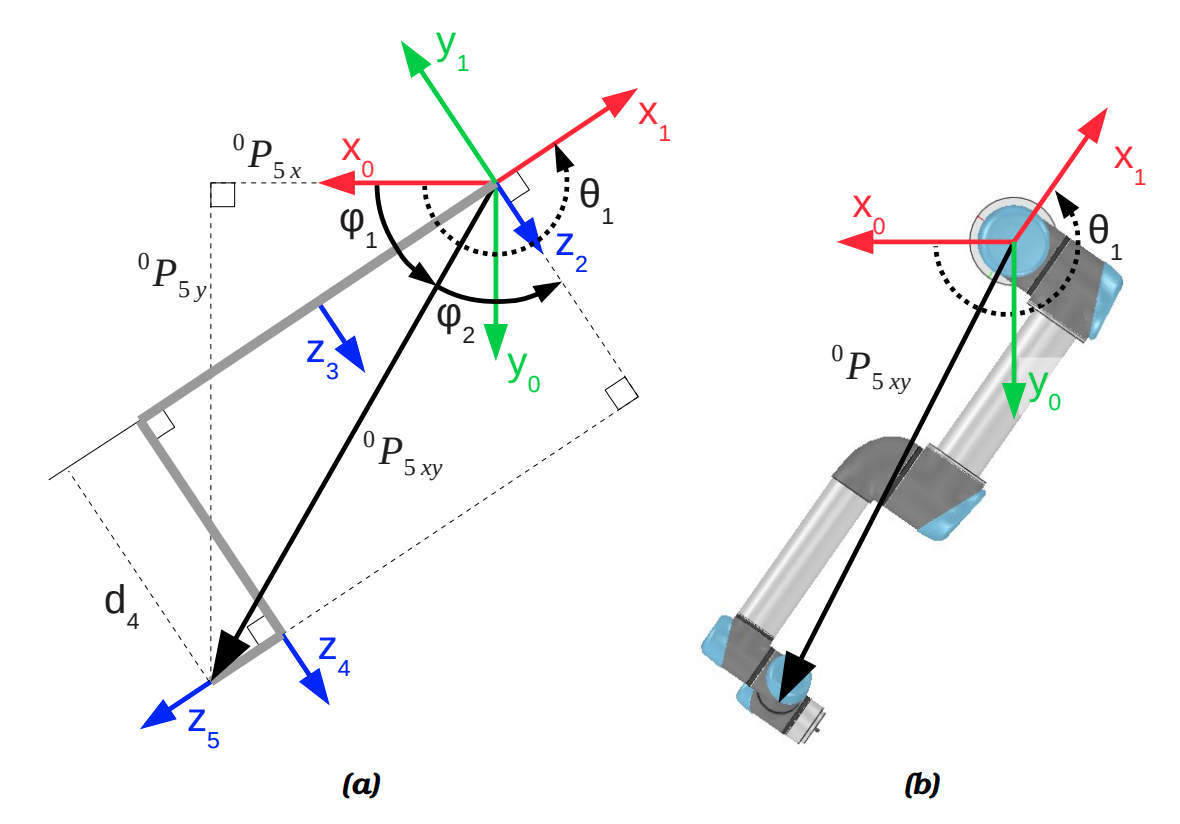
\includegraphics[width = .5\textwidth]{Bilder/inv1}
    \caption{Berechnung von $\theta_1$, Betrachtung von Gelenk eins bis fünf~\cite{rasmusandersenKinematicsUR52018}}\label{fig:inv1-1}
\end{figure}

\subsubsection{2. Gelenk fünf (oberes Handgelenk)}

Im Anschluss kann $\theta_5$ bestimmt werden, da der y-Teil der Position von Gelenk 6 relativ zu Gelenk 1 ($P_{1,6y}$) nur mithilfe von $\theta_5$ und bereits bekannter Parameter $P_{0,6}$, $\theta_1$ und der DH-Parameter berechnet werden kann (siehe Abbildung~\ref{fig:inv1-2}).
Aus dieser Erkenntnis ergibt sich Gleichung~\ref{eq:inv2-1}
$P_{1,6y}$ erhält man durch die Rotation des Ursprungssystems $T_{0,6}$ um die $z_1$-Achse (Gleichung~\ref{eq:inv2-2}).
In Kombination erhält man die Gleichung für $\theta_5$ (Gleichung~\ref{eq:inv2-3}).
Dabei entstehen wiederum zwei Lösungen, die jeweils das Handgelenk ober- oder unterhalb des Arms platzieren.
\begin{equation}
    - P_{1,6y} = d_4 + d_6 \cdot \cos(\theta_5)
    \label{eq:inv2-1}
\end{equation}
\begin{equation}
    P_{1,6y} = - P_{0,6x} \cdot \sin(\theta_1) + P_{0,6y} \cdot cos(\theta_1)
    \label{eq:inv2-2}
\end{equation}
\begin{equation}
    \theta_5 = \pm \arccos \left( \frac{ P_{0,6x} \cdot \sin\theta_1 - P_{0,6y} \cdot \cos\theta_1 - d_4 }{ d_6 } \right)
    \label{eq:inv2-3}
\end{equation}
\begin{figure}[h]
    \centering
    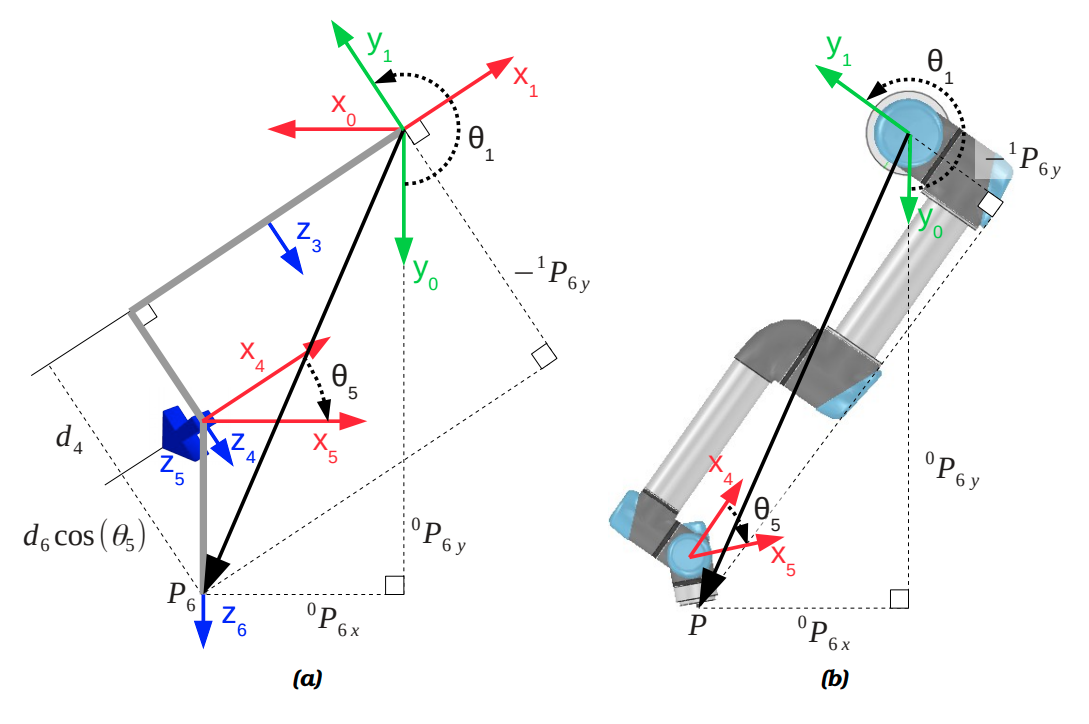
\includegraphics[width = .5\textwidth]{Bilder/inv2}
    \caption{Berechnung von $\theta_5$, Betrachtung von allen Gelenken~\cite{rasmusandersenKinematicsUR52018}}\label{fig:inv1-2}
\end{figure}

\subsubsection{3. Gelenk sechs (Endeffektor)}

Nach $\theta_1$ und $\theta_5$ wird $\theta_6$ bestimmt.
Dazu wird die Eigenschaft des UR5 herangezogen, dass die Z-Achsen von Gelenken zwei, drei und vier stets parallel zur Y-Achse von Gelenk 1 verlaufen (siehe Abbildung~\ref{fig:ur5-axis}).
Deshalb kann die Y-Achse $y_1$ beschrieben von Gelenk sechs ($Y_{6,1}$) aus unabhängig von $\theta_{1,2,3,4}$ betrachtet und mithilfe von sphärischen Koordinaten als Funktion $f(r,\gamma,\phi) = -Y_{6,1}(-\theta_6,\theta_5)$ aufgefasst werden (Radius $r=1$, $-\theta_6$ als Azimuth $\gamma$, sowie $\theta_5$ als polaren Winkel $\phi$; siehe Abbildung~\ref{fig:inv1-3}).
Eine Umrechnung in kartesische Koordinaten ergibt deshalb Gleichung~\ref{eq:inv3-1}, wobei $Y_{6,1}$ mithilfe einer Drehung mit Winkel $\theta_1$ um die Achse $z_1$ beschrieben werden kann (Gleichung~\ref{eq:inv3-2}).
$Z$ und $X$ entsprechen hierbei den Werten der Konvention~\ref{eq:inv-konv}.
Nach Gleichsetzen der x- und y-Einträge der beiden Gleichungen und anschließendem Umformen erhält man $\theta_6$ (Gleichung~\ref{eq:inv3-3}).
Dabei kann es genau eine Lösung geben.
Falls $\sin\theta_5=0$, liegt eine Singularität vor und eine Lösung kann nicht bestimmt werden.
Dies tritt auf, wenn neben den Achsen $z_2$, $z_3$ und $z_4$ auch Achse $z_6$ parallel steht.
In diesem Fall kann eine beliebige Lösung gewählt werden, beispielsweise $\theta_6=0$.

\begin{figure}[h]
    \centering
    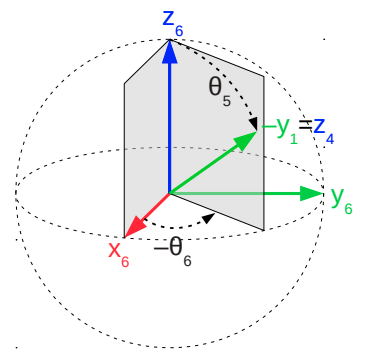
\includegraphics[width = .4\textwidth]{Bilder/inv3}
    \caption{Berechnung von $\theta_6$ mit Sphärischen Koordinaten, für Koordinatensystembeschreibung siehe Abbildung~\ref{fig:ur5-axis}~\cite{rasmusandersenKinematicsUR52018}}\label{fig:inv1-3}
\end{figure}
\begin{equation}
    Y_{6,1}=
    \begin{bmatrix}
        -\sin\theta_5 \cdot \cos\theta_6 \\ \sin\theta_5 \cdot\sin\theta_6 \\ -\cos\theta_5
    \end{bmatrix}
    \label{eq:inv3-1}
\end{equation}
\begin{equation}
    Y_{6,1}=
    -\sin\theta_1\cdot X_{6,0} + \cos\theta_1\cdot Y_{6,0}
    \label{eq:inv3-2}
\end{equation}
\begin{equation}
    \theta_6=
    \arctantwo\left(
    \frac{
        -X_{6,0y} \cdot \sin\theta_1 + Y_{6,0y} \cdot \cos\theta_1
    }{
        \sin\theta_5
    },
    \frac{
        X_{6,0x} \cdot \sin\theta_1 - Y_{6,0x} \cdot \cos\theta_1
    }{
        \sin\theta_5
    }\right)
    \label{eq:inv3-3}
\end{equation}

\subsubsection{4. Gelenk drei (Ellenbogen)}

Die verbleibenden drei Gelenke haben alle parallele Achsen und lassen sich dadurch zu einem zweidimensionalen System vereinfachen (siehe Abbildung~\ref{fig:inv1-4}, rechts).
Um $\theta_3$ zu berechnen kann der Winkel $\phi_3$ zu Hilfe genommen werden (siehe Gleichung~\ref{eq:inv4-1}).
Die Werte $a_2$, $a_3$ sind dabei die DH-Parameter der jeweiligen Gelenke und $\lvert P_{1,4xz} \rvert$ ist der Abstand zwischen Gelenk 1 und Gelenk 4, dessen relative Position bereits bekannt ist.
Aufgrund der Geometrie gilt: $\lvert P_{1,4xz} \rvert \in \lvert a_2 \pm a_3 \rvert$
Nach der Anwendung des $\arccos$ erhält man in der Regel zwei Lösungen, die der Position \enquote{Elbow Up} und \enquote{Elbow Down} entsprechen (Gleichung~\ref{eq:inv4-2}).
\begin{equation}
    \cos(\theta_3) = -cos(\phi_3) = \frac{a_2^2 + a_3^2 - \lvert P_{1,4xz}^2 \rvert}{2 a_2 a_3}   \label{eq:inv4-1}
\end{equation}
\begin{equation}
    \theta_3 = \pm \arccos \left(  \frac{a_2^2 + a_3^2 - \lvert P_{1,4xz}^2 \rvert}{2 a_2 a_3} \right)  \label{eq:inv4-2}
\end{equation}
\begin{figure}[h]
    \centering
    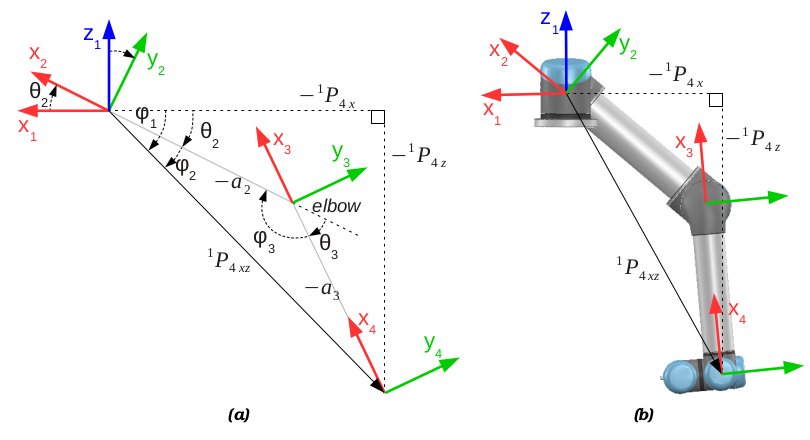
\includegraphics[width = .8\textwidth]{Bilder/inv4}
    \caption{Berechnung von $\theta_4$ durch Vereinfachung als zweidimensionales System und Bestimmung der Transformation zwischen Gelenk 1 und Gelenk 4~\cite{rasmusandersenKinematicsUR52018}}\label{fig:inv1-4}
\end{figure}

\subsubsection{5. Gelenk zwei (Schulter)}

$\theta_2$ kann mithilfe von Abbildung~\ref{fig:inv1-4} ($\theta_2 = \phi_1 - \phi_2$), sowie Gleichung~\ref{eq:inv5-2} und ~\ref{eq:inv5-3} bestimmt werden.
Nach der Substitution von $\phi_3 = \sin(\pi-\theta_3) = \sin(\theta_3)$ erhält man eine Lösung für $\theta_2$ (Gleichung~\ref{eq:inv5-4}).
%\begin{equation}
%    \label{eq:inv5-1}
%\end{equation}
\begin{equation}
    \phi_1 = \arctantwo(-P_{1,4_z}, -P_{1,4x}) \label{eq:inv5-2}
\end{equation}
\begin{equation}
    \phi_2 = \arcsin\left( \frac{-a_3\cdot \sin \phi_3}{\lvert P_{1,4xz}\rvert} \right) \label{eq:inv5-3}
\end{equation}
\begin{equation}
    \theta_2 = \phi_1 - \phi_2 =
    \arctantwo(-P_{1,4_z}, -P_{1,4x}) -
    \arcsin\left( \frac{-a_3\cdot \sin \theta_3}{\lvert P_{1,4xz}\rvert} \right)
    \label{eq:inv5-4}
\end{equation}

\subsubsection{6. Gelenk vier (unteres Handgelenk)}

Der Winkel des letzten Gelenks ist definiert als der Winkel zwischen den Achsen $x_3$ und $x_4$ um Rotationsachse $z_4$ (siehe Definition DH-Parameter, Abschnitt~\ref{sec:dh-konvention}).
Da alle anderen Winkel bereits bekannt sind, kann der letzte Winkel der ersten Spalte $X_{3,4}$ der Transformationsmatrix $T_{3,4}$ entnommen werden.
Mit den ersten beiden Werten dieser Spalte, $X_{3,4x}$ und $X_{3,4y}$, erhält man den Wert von $\theta_4$ (Gleichung~\ref{eq:inv6-1})

\begin{equation}
    \theta_4 = \arctantwo\left( X_{3,4y}, X_{3,4x} \right)    \label{eq:inv6-1}
\end{equation}

\subsubsection{Zusammenfassung}

Mithilfe der Gleichungen~\ref{eq:inv7-1} bis~\ref{eq:inv7-6} kann die Inverse Kinematik eines UR5-Roboters direkt bestimmt werden.
Dabei existieren in der Regel acht mögliche Lösungen, jeweils eine für die Gelenke sechs (Endeffektor), zwei (Schulter) und vier (unteres Handgelenk) und jeweils zwei für die Gelenke eins (Basis), drei (Ellenbogen) und fünf (oberes Handgelenk).
Falls die Achsen $z_2$, $z_3$, $z_4$ und $z_6$ parallel stehen, kann $\theta_6$ beliebig gewählt werden, sodass eine Singularität mit beliebig vielen Lösungen vorliegt.
Neben den DH-Parametern und der gewünschten Transformation des Endeffektors muss für Gleichung~\ref{eq:inv7-1} $P_{0,5}$, für Gleichung~\ref{eq:inv7-3} die Transformation $T_{6,0}$, für Gleichung~\ref{eq:inv7-4} und~\ref{eq:inv7-4} die Transformation $T_{1,4}$ und für Gleichung~\ref{eq:inv7-6} die Transformation $T_{3,4}$ mit der Regeln aus Gleichungen~\ref{eq:inv-rule0},~\ref{eq:inv-rule1} und~\ref{eq:inv-rule2} bestimmt werden.

\begin{equation}
    \theta_1 = \arctantwo(P_{0,5y}, P_{0,5x}) \pm \arccos \left( \frac{d_4}{ \sqrt{ P_{0,5x}^2 + P_{0,5y}^2 }  } \right) + \frac{\pi}{2}
    \label{eq:inv7-1}
\end{equation}
\begin{equation}
    \theta_5 = \pm \arccos \left( \frac{ P_{0,6x} \cdot \sin\theta_1 - P_{0,6y} \cdot \cos\theta_1 - d_4 }{ d_6 } \right)
    \label{eq:inv7-2}
\end{equation}
\begin{equation}
    \theta_6 =
    \arctantwo\left(
    \frac{
        -X_{6,0y} \cdot \sin\theta_1 + Y_{6,0y} \cdot \cos\theta_1
    }{
        \sin\theta_5
    },
    \frac{
        X_{6,0x} \cdot \sin\theta_1 - Y_{6,0x} \cdot \cos\theta_1
    }{
        \sin\theta_5
    }\right)
    \label{eq:inv7-3}
\end{equation}
\begin{equation}
    \theta_3 = \pm \arccos \left(  \frac{a_2^2 + a_3^2 - \lvert P_{1,4xz}^2 \rvert}{2 a_2 a_3} \right)
    \label{eq:inv7-4}
\end{equation}
\begin{equation}
    \theta_2 = \phi_1 - \phi_2 =
    \arctantwo(-P_{1,4_z}, -P_{1,4x}) -
    \arcsin\left( \frac{-a_3\cdot \sin \theta_3}{\lvert P_{1,4xz}\rvert} \right)
    \label{eq:inv7-5}
\end{equation}
\begin{equation}
    \theta_4 = \arctantwo\left( X_{3,4y}, X_{3,4x} \right)
    \label{eq:inv7-6}
\end{equation}

Die Schritte zur Berechnung der inversen Kinematik können für das bessere Verständnis im Code direkt nachvollzogen und visualisiert werden. (?? Referenz)


\section{Singularitäten}\label{sec:singularitaten}

Wie in Abschnitt~\ref{sec:geometrische-losung} ermittelt, existiert beim UR5 genau eine Position, bei der eine Singularität vorliegt.
Singularitäten zeichnen sich dadurch aus, dass es unendlich viele Lösungen für eine bestimmte Zieltransformation gibt.
In der Regel tritt dies genau dann auf, wenn zwei Rotationsachsen parallel zueinander stehen und ihre Bewegung durch das Drehen in gegensätzliche Richtungen beliebig ausgleichen können.

In der Praxis tritt dieser Fall allerdings kaum auf, da durch kleine Rundungsfehler bei der Rechnung nur im Extremfall eine exakte Parallelität hergestellt wird.
Trotzdem sind Singularitäten problematisch, da beim Durchfahren einer solchen Position extreme Positionsänderungen der verschiedenen Gelenke erforderlich sind.
Aus diesem Grund ist es ratsam, diese Positionen möglichst zu vermeiden.
Für weitere Informationen zur Pfadplanung, siehe Abschnitt~\ref{ch:pfadplanung}.
